\documentclass[11pt]{exam}

\usepackage{amssymb, amsmath, amsthm, mathrsfs, multicol, graphicx}
\usepackage{tikz, pgfplots}


\def\d{\displaystyle}
\def\?{\reflectbox{?}}
\def\b#1{\mathbf{#1}}
\def\f#1{\mathfrak #1}
\def\c#1{\mathcal #1}
\def\s#1{\mathscr #1}
\def\r#1{\mathrm{#1}}
\def\N{\mathbb N}
\def\Z{\mathbb Z}
\def\Q{\mathbb Q}
\def\R{\mathbb R}
\def\C{\mathbb C}
\def\F{\mathbb F}
\def\A{\mathbb A}
\def\X{\mathbb X}
\def\E{\mathbb E}
\def\O{\mathbb O}
\def\pow{\mathscr P}
\def\inv{^{-1}}
\def\nrml{\triangleleft}
\def\st{:}
\def\~{\widetilde}
\def\rem{\mathcal R}
\def\iff{\leftrightarrow}
\def\Iff{\Leftrightarrow}
\def\and{\wedge}
\def\And{\bigwedge}
\def\AAnd{\d\bigwedge\mkern-18 mu\bigwedge}
\def\Vee{\bigvee}
\def\VVee{\d\Vee\mkern-18 mu\Vee}
\def\imp{\rightarrow}
\def\Imp{\Rightarrow}
\def\Fi{\Leftarrow}


\def\bar{\overline}

%\pointname{pts}
\pointsinmargin
\marginpointname{pts}
\marginbonuspointname{ bns pts}

\addpoints
\pagestyle{headandfoot}
%\printanswers


\header{MATH 131}{\bf\large Learning Target 18 Quiz}{Fall 2025}
\runningfooter{}{}{Version \version}
\extrafootheight{-.45 in}



\begin{document}
\def\version{A}
%space for name
\noindent {\large\bf Name:} \underline{\hspace{2.5 in}}
\vskip 1em

\begin{questions}
\question Consider the function $f(x) = x^2 + 3$.  Compute the left and right Riemann sums for $f(x)$ with $n = 4$ sub-intervals on the interval $[1,3]$.  Sketch the rectangles whose area represent the \emph{left} Riemann sum on the graph of $f$ below.

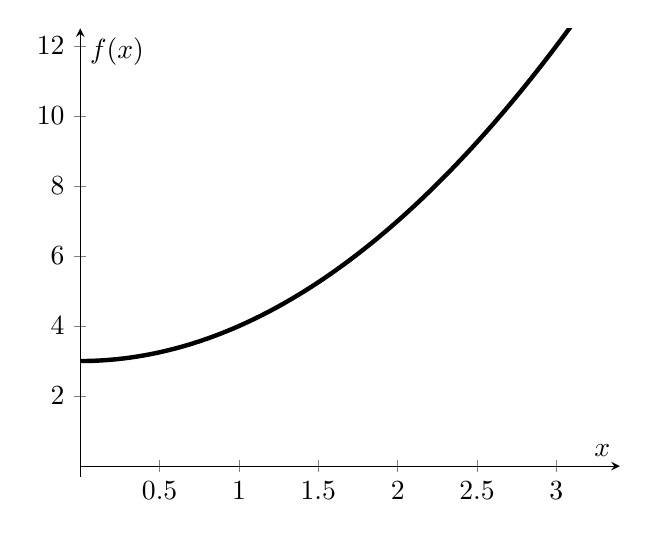
\begin{tikzpicture}[
      declare function={
        func(\x) = \x^2 + 3;
      }
    ]
      \begin{axis}[
        axis x line=middle, axis y line=middle, ymin=-0.3, ymax=12.5, xmin=0, xmax=3.4, xlabel=$x$, ylabel=$f(x)$, grid=none
      ]
        \addplot [domain=0:3.4, samples=100, ultra thick]{func(x)};
      \end{axis}
    \end{tikzpicture}

    Left Riemann sum:
    \vfill
    Right Riemann sum:
    \vfill
\question If the function $f(x)$ above represents the \emph{rate of change} in population, in 100s of people per year, $x$ years after 2025, what do the sums you computed above represent?
\vfill
\vfill
\end{questions}



\newpage

\def\version{B}
%space for name
\noindent {\large\bf Name:} \underline{\hspace{2.5 in}}
\vskip 1em

\begin{questions}
\question Consider the function $f(x) = 12 - x^2$.  Compute the left and right Riemann sums for $f(x)$ with $n = 4$ sub-intervals on the interval $[1,3]$.  Sketch the rectangles whose area represent the \emph{left} Riemann sum on the graph of $f$ below.

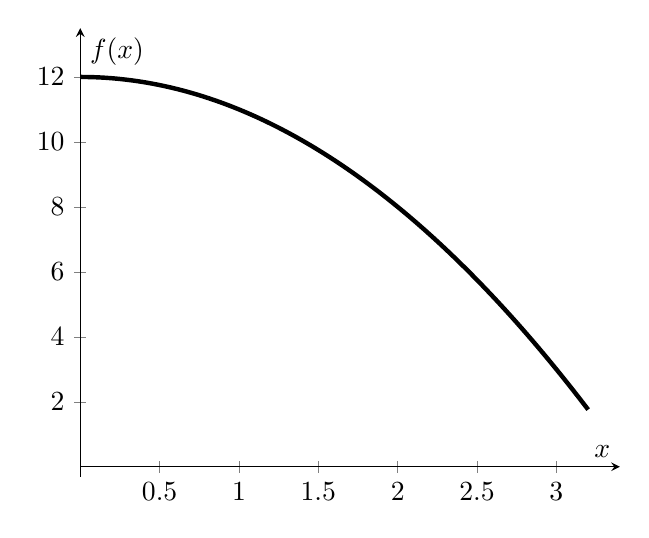
\begin{tikzpicture}[
      declare function={
        func(\x) = 12 - \x^2;
      }
    ]
      \begin{axis}[
        axis x line=middle, axis y line=middle, ymin=-0.3, ymax=13.5, xmin=0, xmax=3.4, xlabel=$x$, ylabel=$f(x)$, grid=none
      ]
        \addplot [domain=0:3.2, samples=100, ultra thick]{func(x)};
      \end{axis}
    \end{tikzpicture}

    Left Riemann sum:
    \vfill
    Right Riemann sum:
    \vfill
\question If the function $f(x)$ above represents the \emph{rate of change} in temperature of a cup of coffee, in degrees per minute, $x$ minutes after it is poured, what do the sums you computed above represent?
\vfill
\vfill
\end{questions}

\newpage

\def\version{C}
%space for name
\noindent {\large\bf Name:} \underline{\hspace{2.5 in}}
\vskip 1em
\begin{questions}
\question Consider the function $f(x) = x^2 - 2x + 4$.  Compute the left and right Riemann sums for $f(x)$ with $n = 4$ sub-intervals on the interval $[1,3]$.  Sketch the rectangles whose area represent the \emph{left} Riemann sum on the graph of $f$ below.

\begin{tikzpicture}[
      declare function={
        func(\x) = \x^2 - 2*\x + 4;
      }
    ]
      \begin{axis}[
        axis x line=middle, axis y line=middle, ymin=-0.3, ymax=10.5, xmin=0, xmax=3.4, xlabel=$x$, ylabel=$f(x)$, grid=none
      ]
        \addplot [domain=0:3.4, samples=100, ultra thick]{func(x)};
      \end{axis}
    \end{tikzpicture}

    Left Riemann sum:
    \vfill
    Right Riemann sum:
    \vfill
\question If the function $f(x)$ above represents the \emph{rate of change} in weight of your pet pig, in lbs per week, $x$ weeks after you adopted her, what do the sums you computed above represent?
\vfill
\vfill
\end{questions}


\newpage

\def\version{D}
%space for name
\noindent {\large\bf Name:} \underline{\hspace{2.5 in}}
\vskip 1em

\begin{questions}
\question Consider the function $f(x) = (x-1.5)^2 + 1$.  Compute the left and right Riemann sums for $f(x)$ with $n = 4$ sub-intervals on the interval $[1,3]$.  Sketch the rectangles whose area represent the \emph{left} Riemann sum on the graph of $f$ below.

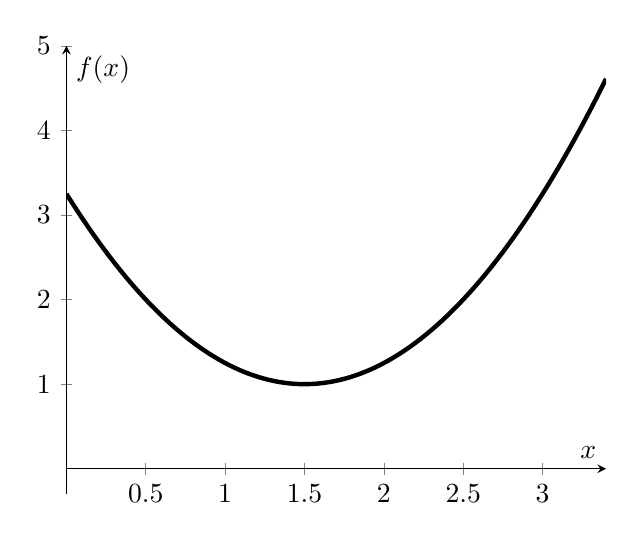
\begin{tikzpicture}[
      declare function={
        func(\x) = (\x - 1.5)^2 + 1;
      }
    ]
      \begin{axis}[
        axis x line=middle, axis y line=middle, ymin=-0.3, ymax=5, xmin=0, xmax=3.4, xlabel=$x$, ylabel=$f(x)$, grid=none
      ]
        \addplot [domain=0:3.4, samples=100, ultra thick]{func(x)};
      \end{axis}
    \end{tikzpicture}
    
    Left Riemann sum:
    \vfill
    Right Riemann sum:
    \vfill
\question If the function $f(x)$ above represents the \emph{rate of change} in weight of your pet emu, in lbs per week, $x$ weeks after you adopted him, what do the sums you computed above represent?
\vfill
\vfill
\end{questions}

\end{document}
